
\section{An Access Control Aware Data Integration Architecture}
\label{sec:prototype}



This section describes the minimal set of components necessary for a data integration and access control enforcement
framework.  It provides an overview of our implementation of each component (based on the languages and models described
in this thesis) and presents an experimental evaluation of our prototype, which focuses on:
%
\begin{inparaenum}[(i)]
\item the \emph{RDB2RDF} data integration;
\item the \emph{reasoning engine}; and
\item the \emph{query engine}.
\end{inparaenum}
%
The aim of this evaluation is simply to show the feasibility of our approach and, although we present different dataset
sizes, at this point we are not looking at improving scalability and thus do not propose any kind of optimisations.
%

We start by presenting a combination of the XSPARQL and AnQL languages, that allows us to query the heterogeneous
sources and create the target Annotated RDF graph.



\subsection{Architecture}


\begin{frame}{Architecture combining XSPARQL and AnQL}

  \begin{center}
    
\begin{tikzpicture}[node distance = 35pt,%
  terminal/.style={ rectangle,minimum size=6mm,rounded corners=3mm,text centered,draw=black!50,fill=gray!20},%
  component/.style={ rectangle,minimum size=6mm,rounded corners=3mm,text centered,draw=black!50},%
  rdb/.style={cylinder, shape border rotate=90, draw,minimum width=1.5cm,minimum height=1cm, shape aspect=.35}%
  ]

  \tikzstyle{every node}=[font=\footnotesize]


  %  reasoner
  \node[terminal, text width=1.5cm, minimum height=1cm] (reasoner) {Reasoner}; %

  \coordinate[left= 5em of reasoner.west] (left-reasoner);

  % domains
  \begin{scope}[node distance = 5pt,text width=1.2cm,anchor=east]
    \node[component] at (left-reasoner) (ac) {Access Control}; %
    \node[component, above=of ac]  (frdf) {Fuzzy}; %
    \node[component,left =of frdf] (trdf) {Temporal}; %
    \node[component,below =of trdf] (prov) {Prove\-nance}; %
  \end{scope}

  % domains outer box
  \node[draw=black,dotted,thick,inner sep=10pt,rectangle,fit=(trdf) (ac) (frdf) (prov)] (domains) {} ;%
  \node[inner sep=0,fill=white] at (domains.north) (domains-label) { \bf Domains};

  \draw[-latex] (reasoner.west) -- (domains.east);%


  \coordinate[right= 5em of reasoner.north east] (right-reasoner);
  % domains
  \begin{scope}[node distance = 5pt,text width=1.1cm,anchor=north west]
    \node[component] at (right-reasoner) (crules) {Custom Rules}; %
    \node[component, above=of crules]  (rhodf) {$\rhodf$}; %
  \end{scope}

  % rules outer box
  \node[draw=black,dotted,thick,inner sep=10pt,rectangle,fit=(rhodf) (crules)] (rules) {} ;%
  \node[inner sep=0,fill=white] at (rules.north) {\bf Rules};

  \draw[-latex] (reasoner.east) -- (rules.west);%


  % anql 
  \node[terminal,text width=1.5cm, above =1em of reasoner] (anql) {AnQL}; %
  \node[draw=black,dotted,thick,inner ysep=15pt,inner xsep=20pt,rectangle,fit=(anql) (reasoner)] (ardf) {} ;%

  \node[doc, above = of anql] (anqlQuery) {AnQL Query}; %
  \draw[-latex] (anqlQuery.south) -- (anql.north);%

  \draw[dashed,-latex] (anqlQuery.west) -| (domains-label.north);%

  \node[inner sep=0,fill=white] at (ardf.north) { \bf Annotated RDFS};


  \draw[latex-] (reasoner.north) -- (anql.south);%


  % input sources
  \documentSetL{below=2.5em of reasoner}{ardf}{Annotated RDF};%

  \draw[dashed,-latex] (ardf.west) -| (domains.south);%
  
  \draw[latex-latex] (reasoner.south) -- (ardf.north);%

 
  


\end{tikzpicture}



%%% Local Variables:
%%% mode: latex
%%% mode: flyspell
%%% mode: reftex
%%% TeX-master: "../thesis"
%%% End:


  \end{center}

\end{frame}



%%% Local Variables:
%%% mode: latex
%%% mode: flyspell
%%% mode: reftex
%%% TeX-master: "../presentation"
%%% End:




%%% Local Variables:
%%% mode: latex
%%% mode: flyspell
%%% mode: reftex
%%% TeX-master: "../presentation"
%%% End:




\subsection{Access Control Enforcement Framework}
\label{sec:fram-descr}

%
\begin{figure}[t]
  \centering
  
\begin{tikzpicture}[node distance = 35pt,scale=.7,transform shape,%
  terminal/.style={ rectangle,minimum size=6mm,rounded corners=2mm,text centered,draw=black!50,fill=gray!20},%
  component/.style={ rectangle,minimum size=6mm,rounded corners=2mm,text centered,draw=black!50},%
  rdb/.style={cylinder, shape border rotate=90, draw,minimum width=1.5cm,minimum height=1cm, shape aspect=.35}%
  ]

  \tikzstyle{every node}=[font=\footnotesize]


  %  reasoner
  \node[terminal, text width=1.5cm, minimum height=1cm] (reasoner) {Reasoner}; %

  \coordinate[left= 5em of reasoner.west] (left-reasoner);

  % domains
  \begin{scope}[node distance = 5pt,text width=1.2cm,anchor=east]
    \node[component] at (left-reasoner) (ac) {Access Control}; %
  \end{scope}

  % domains outer box
  \node[draw=black,dotted,thick,inner sep=10pt,rectangle,fit=(ac)] (domains) {} ;%
  \node[inner sep=0,fill=white] at (domains.north) (domains-label) { \bf Domains};

  \draw[-latex] (reasoner.west) -- (domains.east);%


  \coordinate[right= 5em of reasoner.north east] (right-reasoner);
  % domains
  \begin{scope}[node distance = 5pt,text width=1.1cm,anchor=north west]
    \node[component] at (right-reasoner) (crules) {Custom Rules}; %
    \node[component, below=of crules]  (rhodf) {$\rhodf$}; %
  \end{scope}

  % rules outer box
  \node[draw=black,dotted,thick,inner sep=10pt,rectangle,fit=(rhodf) (crules)] (rules) {} ;%
  \node[inner sep=0,fill=white] at (rules.north) {\bf Rules};

  \draw[-latex] (reasoner.east) -- ($(rules.north west)!(reasoner.east)!(rules.south west)$);%


  % anql 
  \node[terminal,text width=1.5cm, above =1em of reasoner] (anql) {AnQL}; %

  \draw[latex-] (reasoner.north) -- (anql.south);%

  % input sources
  \node[below=2em of reasoner, rdb, align=center]  (ardf)  {Annotated\\ RDF};%


  \draw[latex-latex] (reasoner.south) -- (ardf.north);%

  \node[draw=black,inner sep=10pt,rectangle,fit=(rules) (domains) (anql) (ardf)] (ac) {} ;%
  \node[inner sep=0,fill=white] at (ac.north) (ac-name) { \bf Access Control Enforcement};


  \node[terminal,below =1em  of ac,minimum width=9.5cm] (xsparql) {Data Integration}; %
  \draw[-latex] ($(xsparql.north west)!(ardf.south)!(xsparql.north east)$) -- (ardf.south);%

  \node[terminal,above =1.5em  of ac,minimum width=9.5cm] (anql-rewriter) {Query Rewriter}; %
  \draw[-latex] (anql-rewriter.south) -- (ac-name.north);%

  \node[terminal,above =1.5em  of anql-rewriter,,minimum width=9.5cm] (auth) {Authentication}; %
  \draw[-latex] (auth.south) -- (anql-rewriter.north);%


 
  \node[below=1em of xsparql, rdb]  (crm)  {CRM};%
  \draw[-latex] (crm.north) -- (xsparql.south);%


  \node[left=of crm, rdb]  (hr)  {HR};%
  \draw[-latex] (hr.north) -- ($(xsparql.south west)!(hr.north)!(xsparql.south east)$);%


  \node[right=of crm, rdb]  (dms)  {DMS};%
  \draw[-latex] (dms.north) -- ($(xsparql.south west)!(dms.north)!(xsparql.south east)$);%



\end{tikzpicture}



%%% Local Variables:
%%% mode: latex
%%% mode: flyspell
%%% mode: reftex
%%% TeX-master: "../thesis"
%%% End:


  \caption{RDF Data Integration and Access Control Enforcement Framework}
  \label{fig:systemOverview}
\end{figure}
%
An overview of the proposed framework is depicted in \cref{fig:systemOverview}, which is composed of two main modules:
\emph{Data Integration} and \emph{Access Control Enforcement}.
%
The Data Integration module is responsible for the conversion of existing relational data and access control policies to
\ac{RDF}. Whereas the Access Control Enforcement module caters for the management of access rights and enables
authenticated users to query their \ac{RDF} data.
%
Noticeably, one component we do not tackle in this chapter is the \emph{authentication} component, which can be achieved
by relying on WebId~\cite{SpornyInksterStory:2011aa} and self-signed certificates.
%
The enforcement of the access control is performed by relying on the \emph{query rewriter} component, that expands a
provided SPARQL query with the credentials of the authenticated user.

\subsubsection{Data Integration}
%
The Data Integration module is responsible for the extraction of data and associated access rights from the underlying
relational databases.  The information extracted is subsequently transformed into Annotated \ac{RDF} using the
combination of XSPARQL and AnQL described in \cref{sec:comb-xsparql-anql}.
%
Ideally, the data integration step would be carried out in conjunction with a domain expert, for example to assist in
defining an R2RML~\cite{DasSundaraCyganiak:2011aa} mapping or XSPARQL query that extracts and converts the relational
data into \ac{RDF}.
%
This chapter focusses primarily on retrieving data from relational databases as the enterprise systems we worked with
stored their data in relational format.\footnote{The data and queries presented in this chapter were developed and
  executed in collaboration with a DERI industry partner.  Any data presented here was anonymised.}


\begin{example}[XSPARQL+AnQL]
\label{fig:xsparql-query}

The sample query below demonstrates how information about a project can be extracted from an enterprise timesheet
system.
%
\begin{lstlisting}[basicstyle=\tt\scriptsize,frame=none, numbers=none]
@prefix : <http://urq.deri.org/enterprise#> 
	
for p.Proj_Code, p.Proj_Desc, rp.Res_Code 
from Projects p, ResPrj rp
where p.Proj_Code = rp.Proj_Code
construct { 
	:{$p.Proj_Code} a :Project {fn:concat("[[",$rp.Res_Code,"]]")};
	:Client {$p.Cust_Code} {fn:concat("[[",$rp.Res_Code,"]]")}  } 
\end{lstlisting}
%
The query consists of a \SQLForClause clause that extracts the data from the two underlying relations and the
\ConstructClause in turn is used to generate N-Quads from the results of the database query.

\end{example}


\subsubsection{Access Control Enforcement}

This component is based on our implementation of the Annotated RDFS framework (presented in \cref{fig:aRDF-schema})
where the annotation domain is fixed to access control.
% 
The integrated data retrieved from the original relational databases is stored as Annotated RDF.
%

\paragraph*{Reasoner.}
For this component we consider two distinct forms of inference:
% 
\begin{inparaenum}[(a)]
\item data inference, where new triples are deduced from existing ones (such as the \ac{RDFS} rules); and
\item access rights inference, where new permissions are deduced from existing ones.
\end{inparaenum}
% 
In our prototype, the reasoning component is implemented by the extension of the \ac{RDFS} inference rules presented in
\cref{sec:anql-semantics}.  


In many LOB applications, two forms of hierarchies are considered: 
%
\begin{inparaenum}[(i)]
\item\label{item-entity-hierarchy} hierarchies between entities in the access control annotations; and
\item\label{item-resource-hierarchy} hierarchies between common resources in the data.
\end{inparaenum}
%
Hierarchies of form~\eqref{item-entity-hierarchy} were considered in \cref{sec:modell-access-contr} by adding rules
to the \nrdn program that evaluates the annotations.
%
As for~\eqref{item-resource-hierarchy}, permissions granted to a resource should inherited by all of the resources
children.  Such inheritance chain can be broken by explicitly specifying permissions at a lower level in the tree. 

Considering our access control domain modelling and the use-case of extracting data (and permissions) from their
original sources, one option is to incorporate this business logic into the extraction process.  In this case, the
extraction query must have information on how to propagate the access permissions and apply them to all the necessary
triples.
%
Another option is to use domain specific rules, which our reasoner is capable of processing, in order to propagate the
access permissions or to ensure any domain specific policies.
%
Such rules can be written in a similar way to the Annotated RDFS rules, described in \cref{sec:implementation-notes},
giving us access to the existing data and annotations and allowing us to create new Annotated RDF triples or update
existing ones.


\begin{example}[Domain Specific Rule]
  Consider, in an enterprise scenario, that an existing policy states that if an employee is given access to a
  \uri{Company} record, as per the following triple \triple{C, \typeR, \uri{{:}Company}}, that employee should be given
  access to all triples regarding that company. Such a policy can be enforced by using the following rule:
  %
  \[
  \frac{ 
    \fuzzyg{\triple{C, \typeR, \uri{{:}Company}}}{\lambda_{1}},\ \fuzzyg{\triple{C, P, O}}{\lambda_{2}} 
  }{ 
    \fuzzyg{\triple{C, P, O}}{\lambda_{1} \oplus_{ac} \lambda_{2}} } \enspace ,
  \]
  where~$C, P, O$ and~$\lambda_{1}, \lambda_{2}$ are variables.
  %
  Applying this rule to the sample dataset presented in Figure~\ref{fig:ardf-ac}, would cause the access permission of
  the triple~$\fuzzyg{\triple{\uri{{:}westportCars, \typeR, \uri{{:}Company}}}}{[[jb]]}$ to be propagated to the second
  triple, yielding the following new annotated triple: 
  %
  $$\fuzzyg{\triple{\uri{{:}westportCars, \uri{{:}netIncome}, 1000000}}}{[[jb]]} \enspace .$$
  %
\end{example}




\begin{comment}
  Consider we know from the original system modelling that if a user is given permission to a \uri{{:}Website} he should
  also have access to any of its descendants (connected by the \uri{{:}hasParent} relation).  The following rule can be
  applied to the Annotated RDFS dataset presented in \cref{fig:ardf-ac} to achieve the desired effect:
  %   
  $$\frac{ 
    \fuzzyg{\triple{X, \typeR, \uri{{:}Website}}}{\lambda_{1}},\ \fuzzyg{\triple{Y, \uri{{:}hasParent}, X}}{\lambda_{2}},\ \lambda_{1} \preceq
    \lambda_{2},\ \fuzzyg{\triple{Y, \typeR, \uri{{:}Website}}}{\lambda_{3}} }{ \fuzzyg{\triple{Y, \typeR,
        \uri{{:}Website}}}{\lambda_{1} \oplus_{ac} \lambda_{3}} } \enspace.$$
  % 
  Intuitively, this rule propagates the access control annotation from the parent \uri{{:}Website} to its direct
  descendent.  The exhaustive application of this rule, again in a similar fashion to the RDFS rules, provides the
  intended result of propagating the annotation to all the descendants of a \uri{{:}Website}.

  However, the previous rule is only propagating the permissions to the descendants of \uri{{:}Website} if the
  credentials also allow access to the \uri{{:}hasParent} relation (represented by the~$\lambda_{1} \preceq \lambda_{2}$
  condition).
  % 
  If we want to automatically propagate the annotations from a \uri{{:}Website} to their \uri{{:}hasParent} relations,
  the following rule can be used:
  % 
  $$\frac{\fuzzyg{\triple{X, \typeR, \uri{{:}Website}}}{\lambda_{1}},\ \fuzzyg{\triple{Y, \uri{{:}hasParent},X}}{\lambda_{2}}}
  { \fuzzyg{\triple{Y, \uri{{:}hasParent}, X}}{\lambda_{1} \oplus_{ac} \lambda_{2}} } \enspace.$$

  The previous rules were only rely on information present in the annotation values for the expansion. It is possible
  however, to consider cases where such application specific rules must rely on combining information present in the
  triple with information from the annotation value.  Consider for example the case where the RDF data contains also
  information regarding employee supervision: one rule might be to provide supervisors with access to the triples their
  subordinates are allowed to access:
  % 
  $$\frac{ \fuzzyg{\triple{X, \uri{{:}hasSupervisor}, Y}}{\lambda_{1}},\ \fuzzyg{\triple{S, P, O}}{\lambda_{2}},\ X \in
    \lambda_{2} }{ \fuzzyg{\triple{S, P, O}}{\mathit{extend}(\lambda_{2},X, Y)} } \enspace.$$
  % 
  In this case, the resulting annotation will not be a direct result of applying the $\otimes_{ac}$ or $\oplus_{ac}$
  functions but will also involve extending the original annotation with another element of the annotation
  elements~$\mathbb{ET}$, represented by the function $\mathit{extend}(\lambda,X, Y)$.
  % 
  To realise this rule, the domain must define the necessary functions:
  \begin{inparaenum}[(i)]
  \item $X \in \lambda$ consists of checking if the annotation element $X$ is included in the propositional formula
    $\lambda$; and
  \item $\mathit{extend}(\lambda,X, Y)$ replaces each occurrence of $X$ in $\lambda$ with $X \lor Y$ and performs the
    normalisation of the resulting annotation.
  \end{inparaenum}

\end{comment}




\subsubsection{Query Rewriter}


It is possible to use AnQL directly to query RDF data annotated with access control information, as presented in
\cref{sec:anql-ac-query}. However, allowing the end user to perform AnQL queries is not secure since one could bypass
the access control due to the lack of enforcement of the supplied credentials.

Our proposed solution for the enforcement of the access control is based on query rewriting.  The user is allowed to
write SPARQL queries and the system transparently extends each triple pattern of the provided query with the user
credentials as annotation value, thus generating an AnQL query.  This generated AnQL query is then executed against the
Annotated RDF graph, which guarantees that the user can only access the triples based on the credentials provided.
%
This query rewriting step relies on information provided by the external authentication system: a user session
represents information regarding an authenticated user in the system and contains, among others, the user credentials.
%
The user credentials should be represented as an annotation control element and thus can be easily added into any SPARQL
\ac{BGP} to obtain an AnQL \ac{BAP}.
%






\subsection{Experimental Evaluation}
\label{sec:evaluation}

The benchmark system is a virtual machine, running a 64-bit edition of Windows Server 2008 R2 Enterprise, located on a shared server. 
%
The virtual machine has an Intel(R) Xeon(R) CPU X5650 @ 2.67GHz, with 4 shared processing cores and 5GB of dedicated memory. 
%
For the evaluation we extract both the data and the access rights from two separate software application databases using
XSPARQL.
%
The different datasets ($DS_1$, $DS_2$, $DS_3$, and $DS_4$) use the same databases, tables, and XSPARQL queries and
differ only on the number of records that are retrieved from the databases.
%
\cref{fig:xsparql-evaluation} provides a summary of each dataset, stating the number of database records queried,
the number of triples generated, and the size of the N-Quads representation of the triples.
%
Furthermore, \cref{fig:xsparql-evaluation} includes the run time of the data extraction process and the run time of
importing the data into our Prolog implementation. \cref{fig:load-query-times} provides a high level overview of
the times for each of the datasets.
%

\begin{table} [t]
\centering
\caption{Access Control dataset description}
\label{tab:dataset-description}
\begin{tabular}{lllll}
\toprule
& $DS_1$  & $DS_2$  & $DS_3$  & $DS_4$  \\
\midrule
\emph{database records} & 8854 & 16934 & 33095  & 65417    \\
\emph{triples} & 44775  & 88300 & 175345 & 349430    \\
\emph{file size (MB)} & 6.1 & 12.1 & 23.7  & 47.6   \\
\bottomrule
\end{tabular}
\end{table}

\begin{table} [t]
\centering
\caption{Access Control dataset generation and load times}
\label{fig:xsparql-evaluation}
\begin{tabular}{lllll}
\toprule
& $DS_1$  & $DS_2$  & $DS_3$  & $DS_4$  \\
\midrule
\emph{RDB2RDF (sec)} & 26 & 42  & 82  &  153 \\
\emph{Import (sec)} & 2.69  & 4.74  &  9.17 & 18.94  \\
\bottomrule
\end{tabular}
\end{table}

Based on this simple experiment we have hints that the extraction process and the loading of triples into Prolog behave
linearly but more data intensive tests are still required. As the inferencing times are highly dependent on both the
rules and the data further experimentation is required in this area.


As for the evaluation of the AnQL engine we used the following queries, denoted $Q_1$, $Q_2$, and $Q_3$:
%
\begin{description}[noitemsep]
\item [$Q_1$:] we retrieved all data
  %
  \begin{lstlisting}[basicstyle=\tt\small,mathescape,frame=none,numbers=none]
SELECT * WHERE { ?s ?p ?o ?$\lambda_{1}$ } 
  \end{lstlisting}

\item [$Q_2$:] we queried the data for a specific user 
  %
  \begin{lstlisting}[basicstyle=\tt\small,frame=none,numbers=none]
SELECT * WHERE { ?s ?p ?o "[[jb]]" } 
  \end{lstlisting}

\item [$Q_3$:] we queried the data for a specific role
  %
  \begin{lstlisting}[basicstyle=\tt\small,frame=none,numbers=none]
SELECT * WHERE { ?s ?p ?o "[[:administrators]]" } 
  \end{lstlisting}

\end{description}
% 
The evaluation results of these three queries over the different datasets is presented in
\cref{fig:anql-evaluation} and depicted in Figure~\ref{fig:load-query-times}.
%
These results calculated as an average of 3 response times and show an overhead for the evaluation of annotations $Q_2$
and $Q_3$.


\begin{table} [t]
\centering
\caption{Query execution time in seconds for the different Access Control datasets.}
\label{fig:anql-evaluation}
\begin{tabular}{lllll}
\toprule
& $DS_1$  & $DS_2$  & $DS_3$  & $DS_4$  \\
\midrule
$Q_1$ & 0.06  & 0.14   & 0.28   & 0.42   \\
$Q_2$ & 0.14  & 0.27   & 0.59   & 0.86   \\
$Q_3$ & 0.16  & 0.27   & 0.54   & 1.11   \\
\bottomrule
\end{tabular}
\end{table}

\begin{figure*}[t]\scriptsize
  \centering
  \subfloat[Dataset load times]{
    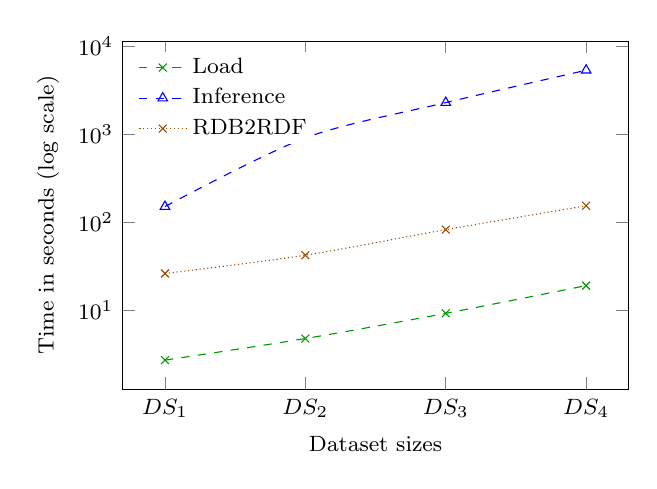
\begin{tikzpicture}
  \begin{loglogaxis}[xlabel={Dataset sizes},ylabel={Time in seconds (log scale)},%
    scaled x ticks = false, x tick label style = {/pgf/number format/fixed},scaled y ticks = false,%
    y tick label style = {/pgf/number format/fixed},enlargelimits=true,xtick={1,2,4,8},%
    xticklabels={$DS_{1}$,$DS_{2}$,$DS_{3}$,$DS_{4}$},log basis x=10,log basis y=10,unbounded coords=jump,xminorticks=false,%
    yminorticks=false,height=6cm,width=8cm,filter discard warning=false,%
    legend style={inner sep=0,legend columns=1,draw=none,font=\tiny,at={(0,0)},anchor=south east,legend pos=north west,anchor=north west,legend cell align=left}]
\addplot[smooth,dashed, color=green!60!black, every mark/.append style={solid},mark=x,] coordinates {
(1, 2.69)
(2, 4.74)
(4, 9.17)
(8, 18.94)
};
\addlegendentry{Load}
\addplot[smooth,dashed, color=blue, every mark/.append style={solid},mark=triangle,] coordinates {
(1, 150)
(2, 906)
(4, 2281)
(8, 5322)
};
\addlegendentry{Inference}
\addplot[smooth,densely dotted, color=orange!60!black, every mark/.append style={solid},mark=x,] coordinates {
(1, 26)
(2, 42)
(4, 82)
(8, 153)
};
\addlegendentry{RDB2RDF}
\end{loglogaxis}\end{tikzpicture}

%%% Local Variables:
%%% mode: latex
%%% mode: flyspell
%%% mode: reftex
%%% TeX-master: "../../thesis"
%%% End:

    \label{fig:load-times}
  }
  \subfloat[Query execution times]{
    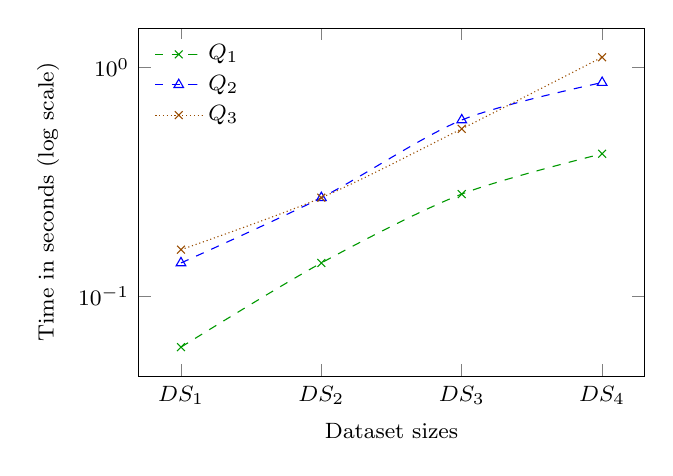
\begin{tikzpicture}
  \begin{loglogaxis}[xlabel={Dataset sizes},ylabel={Time in seconds (log scale)},%
    scaled x ticks = false, x tick label style = {/pgf/number format/fixed},scaled y ticks = false,%
    y tick label style = {/pgf/number format/fixed},enlargelimits=true,xtick={1,2,4,8},%
    xticklabels={$DS_{1}$,$DS_{2}$,$DS_{3}$,$DS_{4}$},log basis x=10,log basis y=10,unbounded coords=jump,xminorticks=false,%
    yminorticks=false,height=6cm,width=8cm,filter discard warning=false,%
    legend style={inner sep=0,legend columns=1,draw=none,font=\tiny,at={(0,0)},anchor=south east,legend pos=north west,anchor=north west,legend cell align=left}]

\addplot[smooth,dashed, color=green!60!black, every mark/.append style={solid},mark=x,] coordinates {
(1, 0.06)
(2, 0.14)
(4, 0.28)
(8, 0.42)
};
\addlegendentry{$Q_{1}$}
\addplot[smooth,dashed, color=blue, every mark/.append style={solid},mark=triangle,] coordinates {
(1, 0.14)
(2, 0.27)
(4, 0.59)
(8, 0.86)
};
\addlegendentry{$Q_{2}$}
\addplot[smooth,densely dotted, color=orange!60!black, every mark/.append style={solid},mark=x,] coordinates {
(1, 0.16)
(2, 0.27)
(4, 0.54)
(8, 1.11)
};
\addlegendentry{$Q_{3}$}
\end{loglogaxis}
\end{tikzpicture}


%%% Local Variables:
%%% mode: latex
%%% mode: flyspell
%%% mode: reftex
%%% TeX-master: "../../thesis"
%%% End:

    \label{fig:query-times}
  }
  \caption{Load and query execution times for the different Access Control datasets}
  \label{fig:load-query-times} 
\end{figure*}


%%% Local Variables:
%%% mode: latex
%%% mode: flyspell
%%% mode: reftex
%%% TeX-master: "../thesis"
%%% End:
